\section{Agents bargain over what the other player can do}
\label{sec:bargaining}

\subsection{Disagreement changes both participation and price}

The agents do not negotiate by simply seeking agreement. Across 526 threads, 920 responses comprise 113 acceptances, 394 counters and 413 rejections. Acceptance is legal for 918 offers. Sol and Opus counter most often, while Gemini and Grok reject most often (Table~\ref{tab:responses}). Yet each accepts between twenty-six and thirty offers. Similar settlement counts therefore coexist with very different forms of disagreement. The low overall acceptance fraction, 113/918, describes selectivity; it does not establish that accepted terms are fair or optimal.

\begin{table}[t]\centering\small
\begin{tabular}{@{}lrrrr@{}}\toprule
Recipient & Responses & Accept & Counter & Reject\\\midrule
Sol &235&30&140&65\\
Gemini &242&26&36&180\\
Opus &189&29&141&19\\
Grok &254&28&77&149\\\bottomrule
\end{tabular}
\caption{All response opportunities. Opus uses action-only recovery in 162 responses. Grok's calls disagree with content in seven acceptances, one counter and three rejections. These are executed response counts under the recorded conditions.}
\label{tab:responses}\end{table}

Offers completing only their author's group are rejected more often than offers completing only the recipient's group: 159/289 versus 38/140. That pooled 27.9-point difference partly reflects negotiation stage. Author-only offers more often open a thread, where rejection is common. Among openings, the contrast is 138/187 versus 31/51, or 73.8\% versus 60.8\%; among later offers it is 21/102 versus 7/89, or 20.6\% versus 7.9\%. Removing one seed block at a time leaves opening differences of 3.0--25.0 percentage points and later differences of 10.0--15.7 points. The later-offer pattern is less concentrated across these blocks, although the remaining offers are selected by earlier bargaining.

This is not a uniform configuration effect. Pooled over stage, the rejection ordering holds for Sol, Gemini and Grok; Opus reverses it and mostly counters both categories. Within stage the ordering holds in five of six Sol/Gemini/Grok cells. Acceptance orderings are less consistent. Table~\ref{tab:offerfull} reports all completion categories. The result is a descriptive relation between the opportunity being offered and the response, not a causal effect of handing a rival a monopoly.

Counters reveal a practice shared across opportunities: preserving goods while negotiating cash. Of 111 counters to author-only completion offers, ninety-two retain all requested deeds; seventy-nine preserve the entire noncash exchange and improve the counterer's cash. In a comparison population of 110 non-completing offers that request a deed and receive a counter, those counts are eighty-seven and eighty-one. Sol and Opus write ninety-two and eighty of these respective populations. Thus repricing the same exchange is common bargaining behavior, not specific evidence of a completion premium. Within the first population, eighty-eight counters still complete only the original author's group, and eighty-five of those demand more cash for the counterer, with a median increase of \$125 across the eighty-eight.

Seller asking prices offer a more direct look at valuation. For each of Sol, Opus and Grok, the median ask relative to board price is higher when the deed would complete the buyer's group, both for mortgaged and unmortgaged deeds (Figure~\ref{fig:prices}). The difference is therefore present within six seller/mortgage cells, not only in a pooled average. Gemini's only comparable cell has one completing-buyer ask and four others; it has the same ordering but little support. The pattern does not survive as a uniform same-asset comparison: among seven same-game, same-seller, same-deed sets with both buyer conditions, four have a higher completing-buyer median, two a lower one and one a tie. Buyer-side bids also differ by system. These results support context-sensitive asking, while leaving the size and source of any completion-specific premium unresolved.

\begin{figure}[t]\centering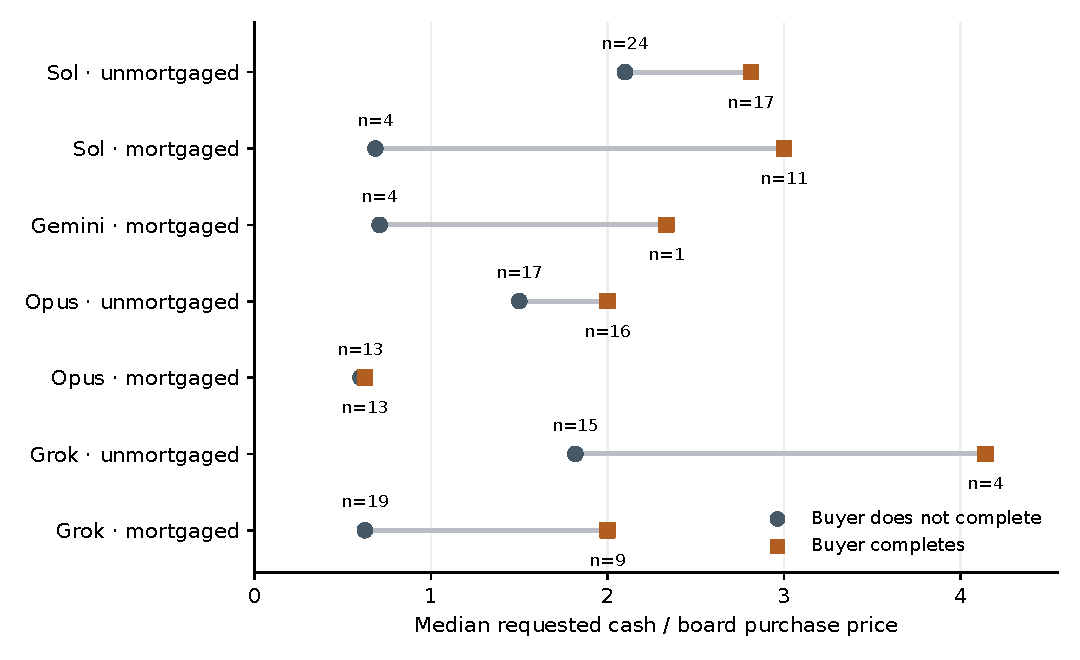
\includegraphics[width=\linewidth]{asking_prices.pdf}
\caption{Median asks for a single deed, divided by board purchase price. Paired points separate whether the buyer would complete a group; labels give offer counts. Mortgage status and seller are held within a row, but deed, recipient, time and negotiation stage can still differ. These are proposed prices, not accepted-price premiums.}
\label{fig:prices}\end{figure}

\subsection{Expressed reasons connect cash to rival development}

The recorded explanations identify the economic considerations behind some refusals. Both LLM-assisted readings find a stated trade-linked consequence for the rival in sixty-one of seventy-four rejections that would complete the recipient's group. This includes 27/38 recipient-only completions and 34/36 offers completing both parties. Gemini and Grok supply fifty-six of the agreed sixty-one; thirty-four records come from G1 and G15. The text concerns rival building budgets, blockers and survival, including trades that would give the rival no new complete group. This is concentrated evidence of strategic attention, not a validated rate of correct opponent modeling.

\TranscriptTitle{g15}{Own completion is refused because the rival could develop sooner}
At G15 turn 63, Sol has \$730 and Grok \$333. Sol offers two greens for Ventnor plus \$100, completing both players' groups. Grok responds:
\TranscriptQuote{fx-g15-refusal-note}
The post-trade balances, \$830 and \$233, agree with the offer ledger. A full first layer of green houses costs \$600, although one legal house costs \$200. Sol removes the cash request and adds Kentucky, then sweetens again. Grok's final public response is:
\TranscriptQuote{fx-g15-final-refusal}
\TranscriptFinding{All three offers fail. Eighteen turns later Grok is eliminated and its blocking deeds pass to Gemini, which wins; Sol never completes either group.}
\TranscriptReading{Grok considers its own new monopoly together with the rival's ability to build. Sol revises terms in response to that objection. The observed reasoning is relational and liquidity-sensitive. The later loss does not tell us whether accepting any of the rejected offers would have been better.}
\TranscriptSource{G15 d168--175, standard responses; quoted public messages are present in the next counterparty requests.}

\TranscriptTitle{g2}{A seller prices the rival's development budget}
At G2 turn 45, Opus holds two yellows and bids \$325 for Sol's Marvin Gardens. Sol counters:
\TranscriptQuote{g2-d124-price}
One turn earlier Sol asked Grok, which owned no yellow, for \$450 for that deed. It now asks Opus for \$650, then \$600. Its note explicitly discusses Opus's post-purchase building funds. The note's \$520 cash remainder is correct; its claim that this buys nine yellow houses is not, because each costs \$150. Opus advertises a final \$450 while retaining a private \$475 contingency; Sol refuses.
\TranscriptFinding{At turn 69 the roles reverse. Opus has \$17 and sells its two yellows to Sol for two railroads plus \$100. Three turns later those railroads pass to Gemini in Opus's bankruptcy. Sol builds on yellow, later sells those buildings, collects \$44 undeveloped rent and no developed yellow rent, and eventually transfers yellow to Gemini through bankruptcy.}
\TranscriptReading{The same deed draws different asks depending on the buyer, and the expressed valuation includes what that buyer could build. Subsequent financial positions reverse who buys the group. The trajectory illustrates why a completed exchange and its final owner must be distinguished.}
\TranscriptSource{G2 d119--128 and d197--198; the undeveloped rent is event 1566. The private ceiling is a recorded contingency, not an estimated reservation value.}

\subsection{Language can bargain, conceal or correct}

Public communication accompanies structured terms. Its strategic role cannot be read from settlement alone: a recipient may accept the price while rejecting the explanation. The next two incidents contrast an agreed bargaining bluff with explicit factual correction.

\TranscriptTitle{g7}{A public final price understates a private contingency}
Sol asks \$625 for North Carolina. Grok counters:
\TranscriptQuote{g7_d42_public}
Its private note retains the higher ceiling:
\TranscriptQuote{g7_d42_private}
\TranscriptFinding{Sol accepts \$600. Grok later completes green by auction but never builds it; after Grok's bankruptcy at turn 110, North Carolina returns to Sol in the green estate. Sol builds on that group two turns later.}
\TranscriptReading{This is an authorized bluff about a bargaining limit, with a settled outcome. G2 provides the contrast of a similar final-price claim that was refused. Neither pair of cases isolates the effect of saying ``final.''}
\TranscriptSource{G7 d41--43; later acquisition event 1680, estate 1946--1954, builds 1971--1973. Sol receives the quoted public message.}

\TranscriptTitle{g19}{The recipient corrects the premise and accepts the terms}
Grok's received call offers Virginia plus \$150 for States and describes a false group-completion benefit:
\TranscriptQuote{g19_d135_false_public}
Both deeds are pink. The same response's note says to abort, and assistant content names an end action. The received proposal nonetheless reaches Sol, which replies:
\TranscriptQuote{g19_d136_correction_accept}
\TranscriptFinding{The deed exchange and \$150 payment execute, completing no group. Sol's note calls the terms favorable.}
\TranscriptReading{Sol separates the bargain from the proposer's false explanation. Acceptance here is evidence of neither credulity nor successful deception. The proposer also has incompatible channels, so the false public claim should not be treated as a coherent plan shared by its whole response.}
\TranscriptSource{G19 d135--136, standard attempts; the false claim is in Sol's delivered request.}
